\section{Scheduling}
\begin{center}
\begin{forest} 
for tree={ edge path={\noexpand\path[\forestoption{edge}] (\forestOve{\forestove{@parent}}{name}.parent anchor) -- +(0,-12pt)-| (\forestove{name}.child anchor)\forestoption{edge label};}
}
[Scheduling
[Unconstrained\\(ASAP),align=center,base=bottom]
[Latency constraint
[Overall Latency\\(ACAP)\\{$\lambda = t_{n} - t_{0}$},align=center,base=bottom]
[Detailed Latency Constraint\\{$ t_j \geq t_i + l_{ij} $}\\{$ t_j \leq t_i + l_{ij} $},align=center,base=bottom]
%[Minimum resource\\under latency,align=center,base=bottom]
]
[Resource constraint 
[Exact algorithms [ILP] [HU'S] ]
[Heuristic algorithm [List Scheduling]]]
]
\end{forest}
\end{center}
Scheduling determines the concurrency of the resulting implementation, and therefore it affects its performance. Therefore the choice of a schedule affects also the area of the implementation. The number of resources may he bounded from above to satisfy some design requirement. For example, a circuit with a prescribed size may have at most one floating point multiplier/divider. When resource constraints are imposed, the number of operations of a given type whose execution can overlap in time is limited by the number of resources of that type.
\begin{center}

\framebox{\Longstack[l]{
- The set of \textbf{operations}: vertex set  $ V= \lbrace v_i;\: i=0, 1, ..., n \rbrace $ \\
- The set of \textbf{dependencies}: set set  $ E= \lbrace (v_i, v_j);\: i, j=0, 1, ..., n; i \neq j \rbrace $ \\
- The set of \textbf{execution delays}:  $ D= \lbrace d_i;\: i=0, 1, ..., n \rbrace $.\\
\, \, The execution delays of the source and sink vertices are both zero: $ d_0 = d_n = 0 $ \\
- The set of \textbf{start time} for the operations:  $ T= \lbrace t_i;\: i=0, 1, ..., n \rbrace $ \\
- The set of \textbf{resources}: $ A= \lbrace a_i;\: i=0, 1, ..., n \rbrace $}}
\end{center}

The  \textit{latency} of the schedule is the number of cycles to execute the entire schedule, or equivalently the difference in start time of the sink and source vertices:  $\lambda = t_{n} - t_{0}$.  Without loss of generality, in our examples we assume  $t_{0} = 1$,  i.e., the first operations start execution in  the first cycle.\\
The sequencing graph requires that the start time of an operation is at least as large as the start time of each of its direct predecessor plus its execution delay, that the following relations hold:
\[t_{i} \geq t_{j} + d_{j}\]
\begin{figure}[H]
    \centering
    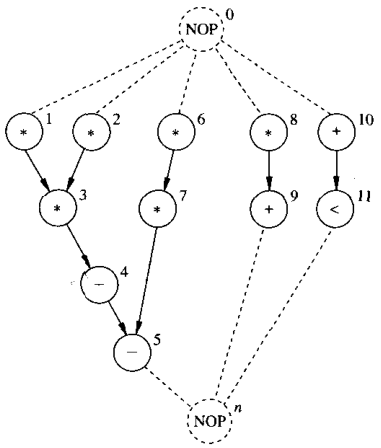
\includegraphics[width=0.4\textwidth]{./Cap4/Images/Image01.png}
    \caption{Sequencing  graph}
    \label{fig:seqgraph}
\end{figure}

\subsection{Scheduling without resource constraints}
Unconstrained scheduling is applied when dedicated resources are used. Unconstrained scheduling is also used when resource binding is done prior to
scheduling, and resource conflicts are solved by serializing the operations that share the same resource. In this case, the area cost of an implementation is defined before and independently from the scheduling step. A lower bound on latency can be computed by unconstrained scheduling, because the minimum latency of  a  schedule under some resource constraint is obviously at least as large as the latency computed with unlimited resources.

\subsubsection{Unconstrained Scheduling: The ASAP Scheduling Algorithm}
The unconstrained minimum-latency scheduling problem can be solved in polynomial time by topologically sorting the vertices of the sequencing graph. This approach is called in jargon  \textit{as soon as possible}  (ASAP) scheduling, because the start time for each operation is the least one allowed by the dependencies. We denote by  $ t^{S} $  the start times computed by the ASAP.
\begin{figure}[H]
    \centering
    \begin{subfigure}[b]{0.5\textwidth}
        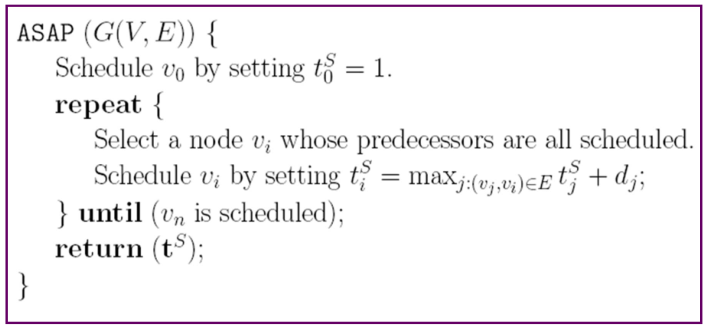
\includegraphics[width=\textwidth]{./Cap4/Images/Image05.png}
        \caption{ASAP algorithm}
   		\label{fig:ASAPAlg}
    \end{subfigure}
    \quad\quad\quad
    \begin{subfigure}[b]{0.4\textwidth}
        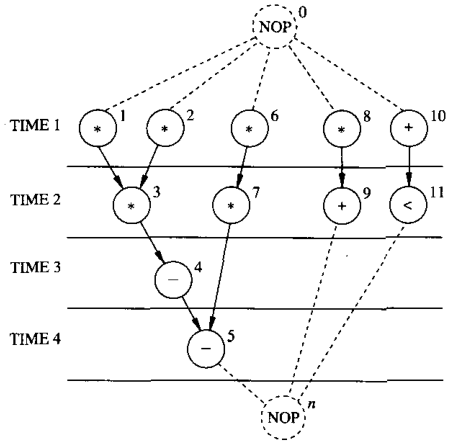
\includegraphics[width=\textwidth]{./Cap4/Images/Image02.png}
        \caption{ASAP schedule}
   		\label{fig:ASAPSch}
    \end{subfigure}
\end{figure}

\paragraph{Example}
Assume all operations have unit execution delay. The ASAP algorithm would set first  $ t_0^{S} = 1 $. Then, the vertices whose predecessors have been scheduled are:
\begin{center}
\begin{tabular}{|l|l|}
  \hline
  \multirow{5}{*}{At T = 1 the ready operation are $ \lbrace v_1, v_2, v_6, v_8, v_{10} \rbrace $} 
  & $ t_1^{S} = max \lbrace t_0^{S} \rbrace + d_0 = 1 $ \\
  & $ t_2^{S} = max \lbrace t_0^{S} \rbrace + d_0 = 1 $ \\
  & $ t_6^{S} = max \lbrace t_0^{S} \rbrace + d_0 = 1 $ \\
  & $ t_8^{S} = max \lbrace t_0^{S} \rbrace + d_0 = 1 $ \\
  & $ t_{10}^{S} = max \lbrace t_0^{S} \rbrace + d_0 = 1 $ \\
  \hline
  \multirow{5}{*}{At T = 2 the ready operation are $ \lbrace v_3, v_7, v_9, v_{11} \rbrace $} 
  & $ t_3^{S} = max \lbrace t_1^{S}, t_2^{S} \rbrace + d_{1} = 2 $ \\
  & $ t_7^{S} = max \lbrace t_6^{S} \rbrace + d_6 = 2 $ \\
  & $ t_9^{S} = max \lbrace t_8^{S} \rbrace + d_8 = 2 $ \\
  & $ t_{11}^{S} = max \lbrace t_{10}^{S} \rbrace + d_{10} = 2 $ \\
  \hline
  At T = 3 ... And so on. & \\
  \hline
\end{tabular}
\end{center}
Note that the start time of the sink  $ t_n^{S} = 5 $, and thus latency is  $\lambda = t_{n} - t_{0}= 5-1 = 4$.
\bigskip

\subsubsection{Latency-Constrained Scheduling: The ALAP Scheduling Algorithm}
We consider now the case in which a schedule must satisfy an upper bound on the latency, denoted by $  \overline{\lambda} $.  This problem may be solved by executing the ASAP scheduling algorithm and verifying that $ (t^{S}_{n} - t^{S}_{0}) \leq \overline{\lambda}$. If a schedule exists that satisfies the latency bound $  \overline{\lambda} $,  it is possible then to explore the range of values of the start times of the operations that meet the bound.\\
The ASAP scheduling algorithm yields the minimum values of the start times.  A  complementary algorithm, the  \textit{as late as possible } (ALAP)   provides the corresponding maximum values. We denote by  $ t^{L} $  the start times computed by the ALAP algorithm.\\
An important quantity used by some scheduling algorithms is the  \textit{mobility}  (or \textit{slack})  of an operation, corresponding to the difference of the start times computed by the ALAP and ASAP algorithms.
\[\mu_{i}=t^{L}-t^{S}; i=0,1,...,n  \]
\begin{figure}[H]
    \centering
    \begin{subfigure}[b]{0.5\textwidth}
        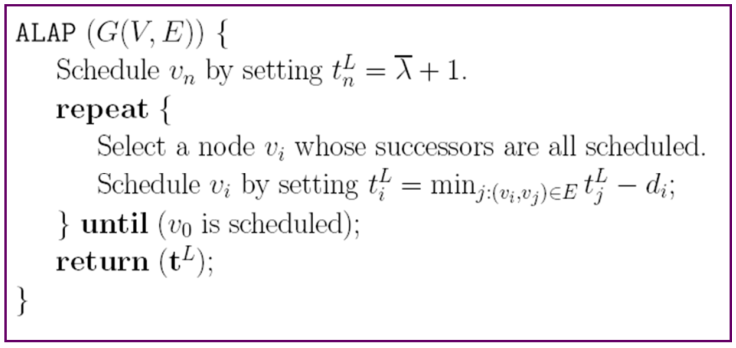
\includegraphics[width=\textwidth]{./Cap4/Images/Image06.png}
        \caption{ALAP algorithm}
   		\label{fig:ALAPAlg}
    \end{subfigure}
    \quad\quad\quad
    \begin{subfigure}[b]{0.4\textwidth}
        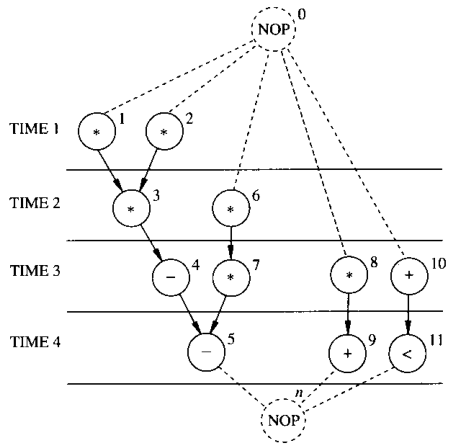
\includegraphics[width=\textwidth]{./Cap4/Images/Image03.png}
        \caption{ALAP  schedule under  latency constraints  of  four  step}
   		\label{fig:ALAPSch}
    \end{subfigure}
\end{figure}

\paragraph{Example}
Assume $ \overline{\lambda} = 4 $. The  algorithm would set first $ t_n^{L} = 5 $. Then, the vertices whose successors have been scheduled are:
\begin{center}
\begin{tabular}{|l|l|}
  \hline
  \multirow{3}{*}{At T = 4 the ready operation are $ \lbrace v_5, v_9, v_{11} \rbrace $} 
  & $ t_5^{L} = min \lbrace t_n^{L} \rbrace - d_5 = 4 $ \\
  & $ t_9^{L} = min \lbrace t_n^{L} \rbrace - d_9 = 4 $ \\
  & $ t_{11}^{L} = min \lbrace t_n^{L} \rbrace - d_{11} = 4 $ \\
  \hline
  \multirow{5}{*}{At T = 3 the ready operation are $ \lbrace v_4, v_7, v_8, v_{10} \rbrace $} 
  & $ t_4^{L} = min \lbrace t_5^{L} \rbrace - d_4 = 3 $ \\
  & $ t_7^{L} = min \lbrace t_5^{L} \rbrace - d_7 = 3 $ \\
  & $ t_8^{L} = min \lbrace t_9^{L} \rbrace - d_8 = 3 $ \\
  & $ t_{10}^{L} = min \lbrace t_{11}^{L} \rbrace - d_{10} = 3 $ \\
  \hline
  At T = 2 ... And so on. & \\
  \hline
\end{tabular}
\end{center}
Note that at the end:  $ t_0^{L} = min \lbrace t_1^{L}, t_2^{L}, t_6^{L}, t_8^{L}, t_{10}^{L} \rbrace - d_0 = min \lbrace 1, 1, 2, 3, 3 \rbrace - d_0 = 1 $
\bigskip \\
$ \mu_{i}= 0 $ implies that  an  operation can  be  started only at one  given  time step in order to meet the overall latency constraint. When the mobility is larger  than zero, it measures the span of the time interval in which it may  be  started.\\
In other words, all the operations with $ \mu_{i}= 0 $ identify the \textit{critical path} because them can't be moved.
\begin{itemize}
\item Operations with $ \mu_{i}= 0: \lbrace v_1, v_2, v_3, v_4, v_5 \rbrace $
\item Operations with $ \mu_{i}= 1: \lbrace v_6, v_7 \rbrace $
\item Operations with $ \mu_{i}= 2: \lbrace v_8, v_9, v_10, v_11 \rbrace $
\end{itemize}
\begin{figure}[H]
    \centering
    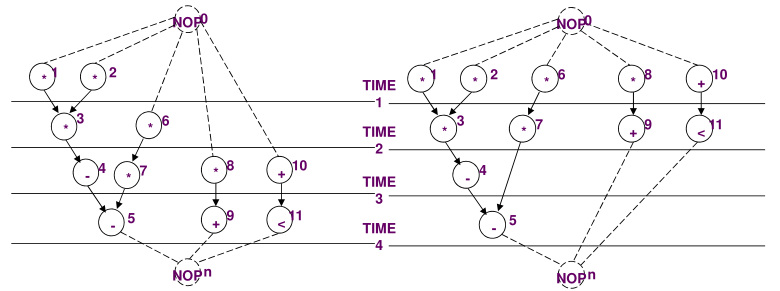
\includegraphics[width=0.7\textwidth]{./Cap4/Images/Image04.png}
    \caption{ALAP and ASAP  schedules}
    \label{fig:ALAPASAP}
\end{figure}

\subsubsection{Scheduling Under Detailed Timing Constraints}
The scheduling problem under latency constraints can be generalized to the case in which  \textit{deadlines}  need to  be  met by other operations. The  deadlines is nothing but \textit{absolute constraints} on the  start  time of the operations.\\
A further generalization is considering  \textit{relative  timing constraints} that bind the time separation between operations pairs, regardless of their absolute value. Relative constraints are very useful in hardware modeling, because the absolute start times are not known \textit{a priori}. \textit{Minimum timing constraints} between any two operations can be used to ensure that an operation follows another by at least a prescribed number of time steps. It is often also important to limit the maximum distance in time between two operations by means of \textit{maximum timing constraints}. The combination of maximum and minimum timing constraints permits us to specify the exact distance in time between two operations and, as a special case, their simultaneity.\\
\textbf{Relative timing constraints} are positive integers specified for some operation pair $ v_i, v_j $.
\begin{itemize}
\item A  \textbf{minimum} timing constraint  $ l_{ij} \geq 0 $  requires:  $ t_j \geq t_i + l_{ij} $
\item A  \textbf{maximum} timing constraint  $ u_{ij} \geq 0 $  requires:  $ t_j \leq t_i + l_{ij} $
\end{itemize}
A  modeling of minimum and maximum timing constraints can be done by means of a constraint graph , that is, an edge-weighted directed graph derived from the sequencing graph.\\
The weight on the edge  ($ v_i, v_j $)  is denoted by  $ w_{ij} $.  Additional edges are related to the timing constraints. For every \textit{minimum timing constraint}  $ l_{ij} $,  we add a  \textit{forward}  edge  in the constraint graph with weight equal to the minimum value, i.e., $ w_{ij} = l_{ij} $.  For every \textit{maximum timing constraint}  $ u_{ij} $,  we add  a  \textit{backward}  edge in the constraint graph with weight equal to the opposite of the maximum value, i.e., $ w_{ij} = - u_{ij} $.\\
A criterion to determine the existence of a schedule is to consider in turn each maximum timing constraint  $ u_{ij} $. Any cycle in the constraint graph including edge $ v_i, v_j $ must have \textit{negative or zero weight}. Therefore, a necessary condition for the existence of the schedule is that the constraint graph does not have positive cycles.

\paragraph{Example}
Consider the example in Figure \ref{fig:relatTimngConst}.  We assume one cycle for addition and two for multiplication.  A  minimum timing constraint requires operation  $ v_4 $  to execute at least  $ l_{04} = 4 $ cycles after operation  $ v_0 $  has started.  A  maximum timing constraint requires operation $ v_2 $  to execute at most  $ u_{21} = 3 $  cycles after operation  $ v_1 $,  has started. Note that the constraint graph has  a  backward edge with negative weight ($ -3 $). The existence of the schedule is given by the cycle with negative weight (between $ v_1, v_2 $), i.e $ 2 -3 = -1 $. Therefore, the constraint graph does not have positive cycles.
\begin{figure}[H]
    \centering
    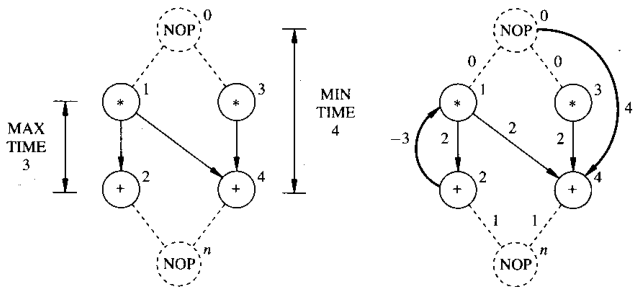
\includegraphics[width=0.6\textwidth]{./Cap4/Images/Image07.png}
    \caption{Example  of  a  consmint  graph,  with  minimum  and  maximum  relative timing  constraints}
    \label{fig:relatTimngConst}
\end{figure}

\subsection{Scheduling with resource constraints}
Scheduling under resource constraints is an important and difficult problem. Resource constraints are motivated by the fact that the resource usage determines the circuit area of resource-dominated circuits. The solution of scheduling problems under resource constraints provides a means for computing the (area latency) trade-off points.

\subsubsection{The Integer Linear Programming Model ILP}
A  formal model of the scheduling problem under resource constraints can be achieved by using binary decision variables with two indices: $ X = \lbrace x_{il}; i=0, 1,...,n;\: l=1, 2,..., \overline{\lambda}+1 \rbrace $. he range of the indexes is justified by the fact that we consider also the source and sink operations and that we start the schedule on cycle  1.  The number  $ \overline{\lambda} $ represents an upper bound on the latency, because the schedule latency is unknown. The bound can be computed by using the ALAP algorithm or a fast heuristic scheduling algorithm, such as a list scheduling algorithm.\\
The indices of the binary variables relate to the operations and schedule steps respectively. In particular, a binary variable,  $ x_{il} $,  is 1 only when operation  $ v_i $  starts in step $ l $ of the schedule, i.e.,  $ l = t_i $.\\
We denote the summations over all operations as $ \sum\limits_i $ and those over all schedule steps as $ \sum\limits_l $.\\
The operations start only once:
\[\sum\limits_l x_{il} = 1,\quad i=0,1,...,n\]
Therefore the start time of any operation $ v_i \in V $ can be stated in terms of  $ x_{il} $  as
\[t_i = \sum\limits_l l \cdot x_{il} \]
The resource bounds must be met at every schedule time step. The number of all operations executing at step $ l $ of type $ k $ must be lower than or equal to the upper bound  $ a_x $.

\paragraph{Example}
Consider the Sequencing graph in the Figure \ref{fig:seqgraphEx}.\\
Constraints:
\begin{itemize}
\item Multiplier: $ a_x=3 \quad d_x=2 $
\item Adder: $ a_+=1 \quad d_1=1 $
\end{itemize}
\begin{figure}[H]
    \centering
    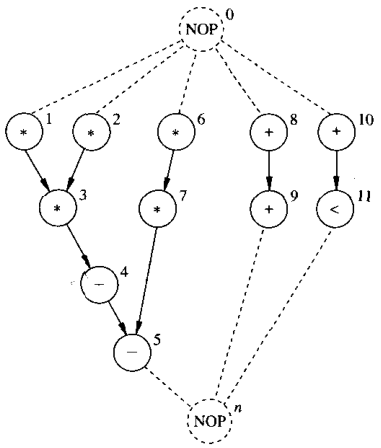
\includegraphics[width=0.35\textwidth]{./Cap4/Images/Image08.png}
    \caption{Sequencing  graph}
    \label{fig:seqgraphEx}
\end{figure}
\begin{center}
\begin{tabular}{l|l|l|l|l}
  \multicolumn{1}{l}{} & \multicolumn{1}{l}{} & \multicolumn{1}{l}{How is ready to be computed} & \multicolumn{1}{l}{List of unfinished operation} & \multicolumn{1}{l}{Operations scheduled} \\
  STEP & k & $ U_{l,k} $ & $ T_{l,k} $ & $ S_{l,k} $ \\
  \hline
  \multirow{2}{*}{$ l=1 $} 
  & * & 1, 2, 6 & / & 1, 2, 6 \\
  & + & 8, 10 & / & 8 \\
  \hline
  \multirow{2}{*}{$ l=2 $} 
  & * & / & 1, 2, 6 & 1, 2, 6 \\
  & + & 9, 10 & / & 10 \\
  \hline
  \multirow{2}{*}{$ l=3 $} 
  & * & 3, 7 & / & 3, 7 \\
  & + & 9, 11 & / & 9 \\
  \hline
  \multirow{2}{*}{$ l=4 $} 
  & * & / & 3, 7 & 3, 7 \\
  & + & 11 & / & 11 \\
  \hline
  \multirow{2}{*}{$ l=5 $} 
  & * & / & / & / \\
  & + & 4 & / & 4 \\
  \hline
  \multirow{2}{*}{$ l=6 $} 
  & * & / & / & / \\
  & + & 5 & / & 5 \\
  \hline
  \multirow{2}{*}{$ l=7 $} 
  & * & / & / & / \\
  & + & / & / & NOP \\
\end{tabular}
\end{center}
$\lambda = t_{n} - t_{0}= 7-1 = 6$
\bigskip \\
The ILP formulation of the constrained scheduling problems is attractive for three major reasons. First it provides an exact solution to the scheduling problems. Second, general purpose software packages can be used to solve the ILP. Last, additional constraints and problem extensions can be easily incorporated. The disadvantage of the ILP formulation is the computational complexity of the problem. The number of variables affect the ability of computer programs to find a solution. Practical implementations of ILP schedulers have been shown to be efficient for medium scale examples hut to fail to solve problems with several hundreds of variables or constraints.

\subsubsection{Hu's Algorithm}
We assume that all operations can he solved by the \textit{same type of resource} and all operations have \textit{unit execution delay}.\\
Despite the simplifications, the \textit{resource-constrained minimum-latency} and \textit{latency-constrained minimum-latency} scheduling problems are  still relevant in architectural synthesis.\\
We compute first a lower bound on the number of resources required to schedule a graph with a latency constraint under these assumptions. We use the sequencing graph model where the source vertex is ignored, because it is irrelevant as far as this problem is concerned.\\
We assume that the sequencing graph is a tree. Under this additional simplification, the problem can  be  solved exactly in polynomial time. We present here the algorithm proposed by Hu for two major reasons. First, Hu's algorithm is one of the few exact polynomial-time algorithms for resource-constrained scheduling. Second, some heuristic algorithms for solving the general scheduling problem are based on Hu's ideas.\\
A  \textbf{labeling}  of a sequencing graph consists of marking each vertex with the weight of its longest path to the sink, measured  in  terms of edges.\\
Let us denote the labels by $ \lbrace\alpha_i;\: i=1, 1, 2,..., n \rbrace $ and let $ \alpha = max \alpha_i $.\\
Let $ p(j) $ be the number of vertices with label equal to $ j $, i.e., $ p(j)=\lbrace v_i \in V : \alpha_i=j \rbrace $. It is obvious that the latency is greater than or equal to the weight of the longest path,
i.e.,  $ \lambda \geq \alpha $.

\paragraph{Example}
Let us consider the graph of Figure \ref{fig:Seqgraph},  where we assume that all operations can  be  executed  by  a general purpose  ALU  with a unit execution delay. A labeled sequencing graph is shown in Figure \ref{fig:LabelSch}.  In this example, $ \alpha = 4 $  and obviously $ \lambda \geq 4 $. Also, $ p(0)=1,\:p(1)=3,\:p(2)=4,\:p(3)=2,\:p(4)=2 $.

\begin{figure}[H]
    \centering
    \begin{subfigure}[b]{0.4\textwidth}
        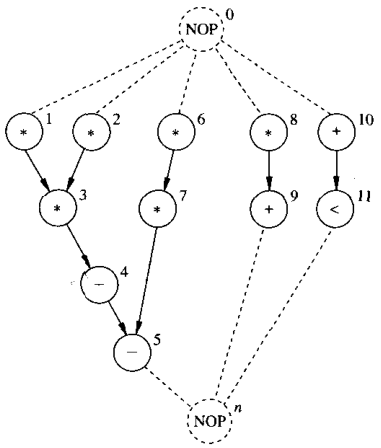
\includegraphics[width=\textwidth]{./Cap4/Images/Image01.png}
        \caption{Sequencing  graph}
   		\label{fig:Seqgraph}
    \end{subfigure}
    \quad\quad\quad
    \begin{subfigure}[b]{0.4\textwidth}
        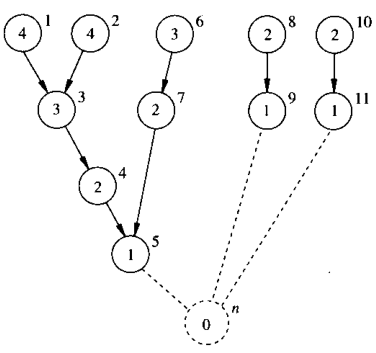
\includegraphics[width=\textwidth]{./Cap4/Images/Image09.png}
        \caption{Labeled  scheduled sequencing graph}
   		\label{fig:LabelSch}
    \end{subfigure}
    \caption{}
\end{figure}

A lower bound on the number of resources to complete a schedule with latency $ \lambda $ is
\[\overline{\alpha} = max \left\lceil \frac{\sum\limits_{j=1}^{\gamma} p(\alpha+1-j)}{\gamma+\lambda-\alpha} \right\rceil \]

\paragraph{Example}
Consider again the previous problem where $ \alpha = 4 $.  Let us compute a resource lower bound to achieve a latency  $ \lambda = 4 $ cycles. Then:
\begin{small}
\[\overline{\alpha} = \left\lceil max \lbrace \frac{p(4)}{1}, \frac{p(4)+p(3)}{2}, \frac{p(4)+p(3)+p(2)}{3}, \frac{p(4)+p(3)+p(2)+p(1)}{4}, \frac{p(4)+p(3)+p(2)+p(1)+p(0)}{5} \rbrace \right\rceil \]
\end{small}
\[ = \left\lceil max \left\lbrace 2,2,\frac{8}{3},\frac{11}{4},\frac{12}{5}  \right\rbrace \right\rceil = 3 \]
where $ \lbrace\gamma = 1,2,...,\alpha + 1\rbrace$.
\begin{figure}[H]
    \centering
    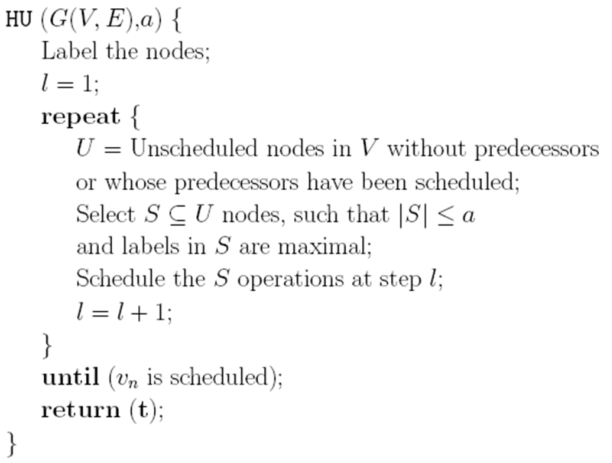
\includegraphics[width=0.4\textwidth]{./Cap4/Images/Image10.png}
    \caption{HU algorithm}
    \label{fig:HUalg}
\end{figure}

\paragraph{Example}
Consider again the previous problem with \textit{hardware resource} $ \overline{\alpha} = 3 $ (no distinction about kind of operations).
\begin{center}
\begin{tabular}{l|l|l}
  \multicolumn{1}{l}{} & \multicolumn{1}{l}{How is ready to be computed}  & \multicolumn{1}{l}{Operations scheduled} \\
  STEP & $ U_{l} $  & $ S_{l} $ \\
  \hline
  $ l=1 $ & 1, 2, 6, 8, 10 & 1, 2, 6 \\
  \hline
  $ l=2 $ & 8, 10, 3, 7 & 3, 7, 8 \\
  \hline
  $ l=3 $ & 10, 4, 9 & 10, 4, 9 \\
  \hline
  $ l=4 $ & 5, 11 & 5, 11 \\
  \hline
  $ l=5 $ &  & NOP \\
\end{tabular}
\end{center}

\subsubsection{Heuristic Scheduling Algorithms: List Scheduling}	
Practical problems in hardware scheduling are modeled by generic sequencing graphs, with (possibly) multiple-cycle operations with different types. With this model, the \textit{minimum-latency}  resource-constrained scheduling problem and the  \textit{minimum-resource} latency-constrained problem are known to  be  intractable. Therefore, heuristic algorithms have been researched and used.\\
We consider first the problem of \textit{minimizing latency} under resource constraints. The algorithm is an extension of Hu's algorithm to handle multiple operation types and multiple-cycle execution delays.
\begin{figure}[H]
    \centering
    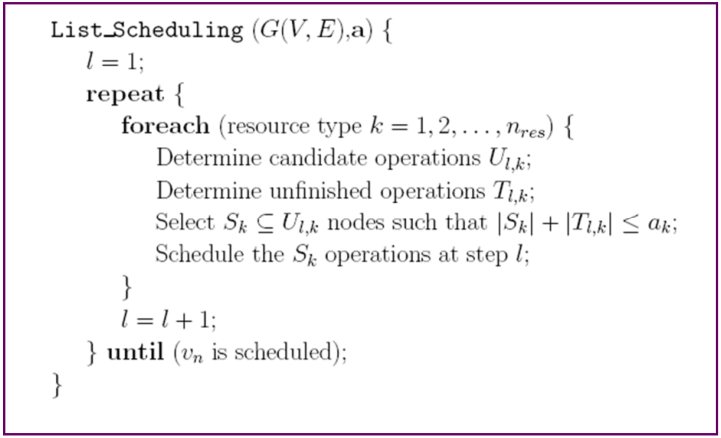
\includegraphics[width=0.4\textwidth]{./Cap4/Images/Image11.png}
    \caption{List scheduling algorithm for minimum latency}
    \label{fig:ListScheHUalg}
\end{figure}
The candidate operations  $ U_{l,k} $ are those operations of type $ k $ whose predecessors have already been scheduled, so that the corresponding operations are completed at step $ l $. The unfinished operations  $ T_{l,k} $ are those operations of type $ k $ that started at earlier cycles and whose execution is not
finished at step $ l $.\\
The computational complexity of the algorithm is  $ O(n) $.  It constructs a schedule that satisfies the resource constraints by construction. However, the computed schedule may \textit{not} have minimum latency.\\
A textit{priority  list } of the operations is used in choosing among the operations, based on some
heuristic urgency measure. A common priority list is to label the vertices with weights of their longest path to the sink and to rank them in decreasing order. The most urgent operations are scheduled first. Note that when the operations have unit delay and when there is only one resource type, the algorithm is the same as \textit{Hu}'s and it yields an optimum solution for tree-structured sequencing graphs. Scheduling under resource and relative timing constraints can be handled by list scheduling.

\paragraph{Example}
Assume we have $ a_1=3 $ multipliers and  $ a_2=1 $  ALU. Let us assume that the execution delays of the multiplier and the ALU are  2  and  I,  respectively.
\begin{figure}[H]
    \centering
    \begin{subfigure}[b]{0.35\textwidth}
        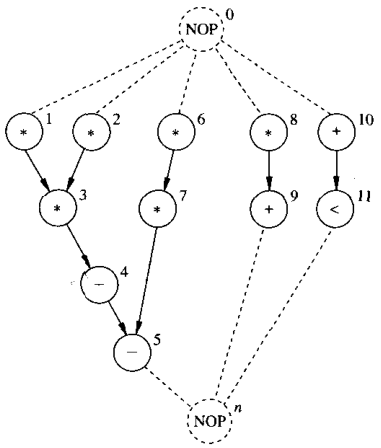
\includegraphics[width=\textwidth]{./Cap4/Images/Image01.png}
        \caption{Sequencing  graph}
   		\label{fig:Seqgraph2}
    \end{subfigure}
    \quad\quad\quad
    \begin{subfigure}[b]{0.35\textwidth}
        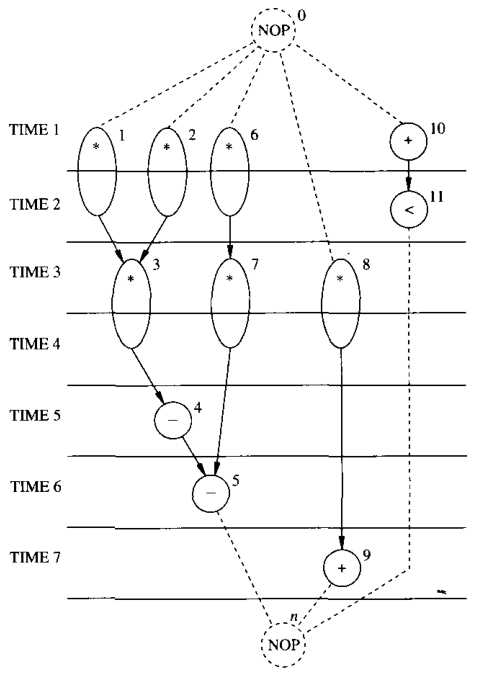
\includegraphics[width=\textwidth]{./Cap4/Images/Image12.png}
        \caption{Scheduled sequencing graph under resource constraints}
   		\label{fig:ListLabelSch}
    \end{subfigure}
    \caption{}
\end{figure}
\begin{center}
\begin{tabular}{l|l|l|l|l}
  \multicolumn{1}{l}{} & \multicolumn{1}{l}{} & \multicolumn{1}{l}{How is ready to be computed} & \multicolumn{1}{l}{List of unfinished operation} & \multicolumn{1}{l}{Operations scheduled} \\
  STEP & k & $ U_{l,k} $ & $ T_{l,k} $ & $ S_{l,k} $ \\
  \hline
  \multirow{2}{*}{$ l=1 $} 
  & * & 1, 2, 6, 8 & / & 1, 2, 6 \\
  & + & 10 & / & 10 \\
  \hline
  \multirow{2}{*}{$ l=2 $} 
  & * & / & 1, 2, 6 & 1, 2, 6 \\
  & + & 11 & / & 11 \\
  \hline
  \multirow{2}{*}{$ l=3 $} 
  & * & 3, 7, 8 & / & 3, 7, 8 \\
  & + & / & / & / \\
  \hline
  \multirow{2}{*}{$ l=4 $} 
  & * & / & 3, 7, 8 & 3, 7, 8 \\
  & + & / & / & / \\
  \hline
  \multirow{2}{*}{$ l=5 $} 
  & * & / & / & / \\
  & + & 4 & / & 4 \\
  \hline
  \multirow{2}{*}{$ l=6 $} 
  & * & / & / & / \\
  & + & 5 & / & 5 \\
  \hline
  \multirow{2}{*}{$ l=7 $} 
  & * & / & / & / \\
  & + & 9 & / & 9 \\
  \hline
  \multirow{2}{*}{$ l=8 $} 
  & * & / & / & / \\
  & + & / & / & NOP \\
\end{tabular}
\end{center}
$\lambda = t_{n} - t_{0}= 8-1 = 7$
\bigskip \\
List scheduling can also be applied to \textit{minimize the resource} usage under latency constraint.  For this problem, the \textit{slack}  of an operation is used to rank the operations, where the slack is the difference between the latest possible start time (computed by an \textit{ALAP} schedule) and the index of the schedule step under consideration ($ s_i $ = start time of the $ v_i $ computed by the ALAP $ - $ STEP $ l $). The lower the slack, the higher the urgency in the list is. Operations with zero slack are always scheduled; otherwise the latency bound would be violated. Scheduling such operations may require additional resources. The remaining operations are scheduled only if they do not require additional resources.
\begin{figure}[H]
    \centering
    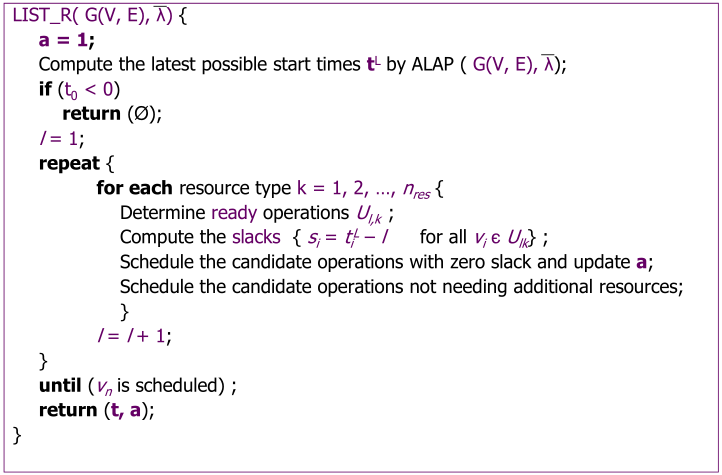
\includegraphics[width=0.6\textwidth]{./Cap4/Images/Image13.png}
    \caption{List scheduling algorithm for minimum resource usage}
    \label{fig:ListScheHUalgminRes}
\end{figure}

\paragraph{Example}
Assume Unit-delay resources. Compute with ALAP the maximum latency: $\lambda = 4$. Start with $ a_1 = 1 $ multiplier and $ a_2 = 1 $ adder.
\begin{figure}[H]
    \centering
    \begin{subfigure}[b]{0.35\textwidth}
        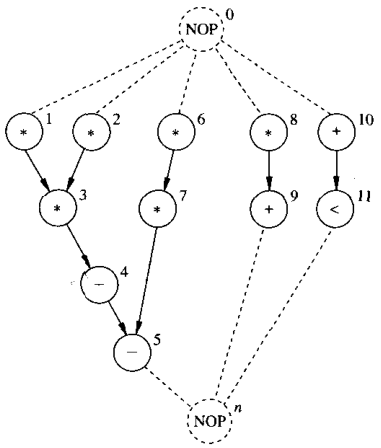
\includegraphics[width=\textwidth]{./Cap4/Images/Image01.png}
        \caption{Sequencing  graph}
   		\label{fig:Seqgraph3}
    \end{subfigure}
    \quad\quad\quad
    \begin{subfigure}[b]{0.4\textwidth}
        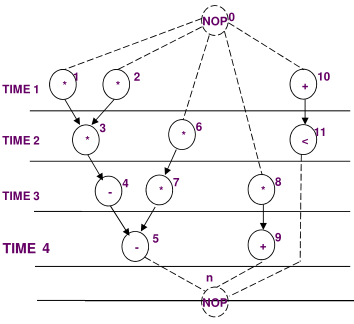
\includegraphics[width=\textwidth]{./Cap4/Images/Image14.png}
        \caption{Scheduled sequencing graph under latency constraint}
   		\label{fig:ListLabelSchLaten}
    \end{subfigure}
    \caption{}
\end{figure}
\begin{center}
\begin{tabular}{l|l|l|l|l|l}
  \multicolumn{1}{l}{} & \multicolumn{1}{l}{} & \multicolumn{1}{l}{How is ready to be computed} &  \multicolumn{1}{l}{} & \multicolumn{1}{l}{Operations scheduled} & \multicolumn{1}{l}{Resources} \\
  STEP & k & $ U_{l,k} $ & Slack & $ S_{l,k} $ & Q \\
  \hline
  \multirow{6}{*}{$ l=1 $} 
  & * & 1, 2, 6, 8 & $ s_1=1-1=0 $ & 1, 2 & $ a_1=1+1=2 $ \\
  & & & $ s_2=1-1=0 $ & & \\
  & & & $ s_2=1-1=0 $ & & \\
  & & & $ s_6=2-1=1 $ & & \\
  & & & $ s_2=3-1=2 $ & & \\
  & + & 10 & $ s_{10}=3-1=2 $ & 10 & $ a_2=1 $ \\
  \hline
  \multirow{4}{*}{$ l=2 $} 
  & * & 8, 3, 6 & $ s_8=3-2=1 $ & 3, 6 & $ a_1=2 $ \\
  & & & $ s_3=2-2=0 $ & & \\
  & & & $ s_6=2-2=0 $ & & \\
  & + & 11 & $ s_{11}=4-2=2 $ & 11 & $ a_2=1 $ \\
  \hline
  \multirow{3}{*}{$ l=3 $} 
  & * & 7, 8 & $ s_7=3-3=0 $ & 7, 8 & $ a_1=2 $ \\
  & & & $ s_8=3-3=0 $ & & \\
  & + & 4 & $ s_4=4-4=0 $ & 4 & $ a_2=1 $ \\
  \hline
  \multirow{3}{*}{$ l=4 $} 
  & * & / & / & / & $ a_1=2 $ \\
  & + & 5, 9 & $ s_5=4-4=0 $ & 5, 9 & $ a_2=1+1=2 $ \\
  & & & $ s_9=4-4=0 $ & & \\
  \hline
  \multirow{2}{*}{$ l=5 $} 
  & * & / & / & / & $ a_1=2 $ \\
  & + & NOP & / & / & $ a_2=2 $ \\
\end{tabular}
\end{center}
At the end the minimum number of resources under latency constraint ($\lambda = 4$) are $ a_1 = 2 $ multipliers and $ a_2 = 2 $ adders.